\newcommand{\cdwM}{\Delta}
\begin{disclaimer}
	Large parts of this chapter are based on the unpublished and so far unfinished manuscript~\cite{Steil:2024RGMF} and related work which has been done in close collaboration with M. Buballa and B.-J. Schaefer.
	The manuscript~\cite{Steil:2024RGMF} is based on research done for this dissertation.
	The draft for~\cite{Steil:2024RGMF} is in its early stages and so far I am the sole contributor to the document in terms of explicit computations and text.
	Parts of \cref{subsec:renomMF} discuss results done in collaboration with L. Kurth.
	
	The numerical results discussed in \cref{sec:cdwmf}, were obtained with various versions of my \Cpp{} code~\cite{Steil:2023QMcpp}, computing the phase diagrams in the $\mu$-$T$-plane in a few hours of wall time using various consumer processors.
\end{disclaimer}

The role of bosonic thermal and quantum fluctuations on the stability of inhomogeneous chiral condensates remains unclear. Recent \frg{} studies, \cf{} \cref{subsec:inhomoLiterature} and especially the discussion surrounding \cref{fig:QMMarno,fig:fuQCDpd,fig:qcdZphis}, have shown indications, that inhomogeneous chiral condensation might be possible beyond the mean-field/large-$N_c$ limit. Both \frg{} studies~\cite{Fu:2019hdw,Tripolt:2017zgc} used indirect methods, related to the stability analysis discussed in \cref{subsec:stability}, to infer information about the possibility of inhomogeneous condensation. 
We plan to contribute to this research in two ways.\bigskip

With the methodological developments regarding both the numerics for \frg{} flow equations, mainly discussed in \cref{chap:zeroONSU2} and \cref{sec:gny_frg,sec:gnyFiniteN}, and the stability analysis, discussed in \cref{sec:gnInfHomo}, we plan to study inhomogeneous phases by means of a \frg{} based stability analysis.
We believe, that we now have the proper tools and understanding to apply our conceptual developments to \loefts{} of \qcd{} in the spirit of \cref{subsec:chiralLEFT}.
With the developed \cfd{} framework for \frg{} flow equations it should be possible to continue the discussion started in \ccite{Tripolt:2017zgc} to answer the question whether there is an instability towards inhomogeneous condensation in the \qmm{} in \lpa{}. 
The main point of interest of \ccite{Tripolt:2017zgc} were thermodynamic instabilities/artifacts of the \qmm{} in \lpa{} and inhomogeneous condensates were not the focus of the discussion in \ccite{Tripolt:2017zgc}. 
A review of the issues discussed in \ccite{Tripolt:2017zgc} can be found in Sec.~III.B of the recent review~\cite{Fu:2022gou}.
Very recent results~\cite{Ihssen:2023xlp} have brought significant progress with a combination of improvements regarding regulator choice, truncation but also importantly a robust \cfd{} formulation of the underlying flow equation.\bigskip

The second way in which we want to contribute to the research into inhomogeneous phases beyond mean-field is to the best of our knowledge original to our work~\cite{Steil:2023RGMF} and this thesis.
We plan to supplement the indirect detection methods with a direct method.
To this end we developed a way to incorporate an explicit inhomogeneous condensate into the \frg{} treatment of \loefts{} like the \qmm{}. We will spend the rest of this chapter discussing this development.

In the next \cref{sec:lpacdw} we will discuss the central result of this chapter, \viz{} our successful derivation of a \lpa{} flow equation for a specific inhomogeneous condensate \dash{} the \acrrepeat{cdw} \dash{} in the \qmm{}. This derivation is based on two related analytical/symbolic ideas, which we will discuss in detail, and a subsequent rather tedious but straight forward symbolic computation. We will include the latter only in the digital auxiliary file~\cite{Steil:2023qmmcdw}.

In the second and last \cref{sec:cdwmf} of this chapter, we will discuss a series of mean-field results we obtained using the derived flow equation.
Here we will just focus on the obtained results rather than the technical details given the already substantial scope of the present work.
Details regarding the implementation and the involved expressions can be found in the \Cpp{} code~\cite{Steil:2023QMcpp}, in the digital auxiliary file~\cite{Steil:2023qmmcdw}, and will eventually be discussed in \ccite{Steil:2023RGMF}.
These studies do not include any bosonic fluctuations and the derived flow equation can be integrated in \rgscale{} symbolically.
We will focus on \rgct{} mean-field computations to study the \qmm{} as a \loeft{} rather than a renormalizable model.

We will not conclude this chapter with its own, separated conclusion and outlook, since it is the last chapter of the main part of this thesis.
We will include our concluding remarks and outlook regarding this part of our research, in the following final summary and outlook in \cref{chap:conclusion}.

\section{Deriving a LPA flow equation for the chiral density wave}\label{sec:lpacdw}
Considering the \qmm{} of \cref{subsubsec:qcdQMM} in \lpa{} entails the ansatz \eqref{eq:QMMeaa} for the \eaa{}:
\begin{align}
\FSeaa_k[\FSmf{\FSsf}]\equiv \intx[x]\,\bigg( 
\MFpsib(\gamma^\nu \partial_\nu -\gamma^4\mu + h \MFphi_i \uIItv^{i} )\MFpsi
+\frac{1}{2}\big(\partial_\mu\MFphi\big)^2
+U_{k}(\MFrho)
\bigg)\,.
\label{eq:QMMlpa}
\end{align}
For the condensates \dash{} the possible solutions of the \qeom{} \dash{} we consider in this section exclusively
\begin{align}
\FSsfEoM{}=\MFEIchi{}=(\MFEIphi(\vec{x}\vts),0,0)\,,
\label{eq:qmmMFEIphi}
\end{align}
with ``the'' \acrrepeat{cdw}
\begin{align}
\MFEIphi(\vec{x}\vts)\equiv \cdwM (\cos(\vec{q}\cdot\vec{x}\vts),0,0,\sin(\vec{q}\cdot\vec{x}\vts))\,,
\label{eq:cdw}
\end{align}
with wave vector $\vec{q}$ and amplitude $\Delta$.
Due to its specific analytic properties this is one of the most commonly studied inhomogeneous modulations, see, \eg{}, \ccite{\cdwHEP} and \cref{sec:inhomogeneousPhases}.
A crucial and unique property of this inhomogeneous modulation is the fact that, its related $O(4)$ invariant is constant:
\begin{align}
\frac{1}{2}\,\MFEIphi(\vec{x}\vts)^2=\frac{1}{2}\cdwM^2=\mathrm{const.}
\label{eq:cdwPyth}
\end{align}
on account of the Pythagorean identity. Another closely related property is a variant of Euler's formula
\begin{align}
\forall O^2=\Id\quad \MFEIphi_0(\vec{x}\vts)\pm \iu O \MFEIphi_3(\vec{x}\vts)=\cdwM\exp(\pm \iu O \vec{q}\cdot\vec{x}\vts)\,.
\label{eq:cdwEuler}
\end{align}
A third very nice property is, that in the limit $\vec{q}=0$ the \cdw{} becomes the ordinary homogeneous condensate
\begin{align}
\MFEIchi{}\stackrel{\vec{q}\,=\,0}{\longrightarrow}\MFEchi{}=((\Delta,0,0,0),0,0)\,.
\label{eq:qmmMFEIphiHom}
\end{align}

When evaluating the Wetterich equation on the \cdw{} background, \cref{eq:cdwPyth} allows for a simple and conventional treatment of the \lpa{} potential on the \rhs{} of the \frgEquation{}.
The \rhs{} involves the fermionic and bosonic two-point functions
\begin{align}
	\FSvertexArg{\FSeaaEoMI}{\MFpsib, \MFpsi}(x,y)&=\delta^{(4)}(x-y)\big[\gamma^\nu\partial_{x^\nu}-\gamma^4\mu +\tfrac{h \Delta}{2}(\cos(\vec{q}\cdot\vec{x}\vts) +2\iu  \gammach t_3 \sin(\vec{q}\cdot\vec{x}\vts))\big]\, ,\label{eq:cdwGF}\\[.4em]
	\FSvertexArg{\FSeaaEoMI}{\MFphi_i, \MFphi_j}(x,y)&=\delta^{(4)}(x-y)\big[(-\delta_x^2+U'_k(\Delta^2/2))\delta_{i,j}+U''_k(\Delta^2/2) \MFEIphi_i(\vec{x}\vts) \MFEIphi_j(\vec{x}\vts)\big]\, ,\label{eq:cdwGB}
\end{align}
which are manifest position-dependent for $q\equiv |\vec{q}\vts|\neq 0 $.
In momentum space this amounts to a non-diagonal coupling of momenta, which is a characteristic feature of inhomogeneous phases. As mentioned in \cref{sec:inhomogeneousPhases}, this non-diagonal structure in momentum space makes an inversion \dash{} necessary for the computation of propagators \dash{} of the involved two-point functions impossible with standard techniques.

The unique analytical properties of the \cdw{} however, here notably \cref{eq:cdwEuler}, make a symbolic inversion possible. Noting that $(2\gammach t_3)^2=\Id$, we may rewrite \cref{eq:cdwGF}
as
\begin{align}
\FSvertexArg{\FSeaaEoMI}{\MFpsib, \MFpsi}(x,y)&=\delta^{(4)}(x-y)\big[\gamma^\nu\partial_{x^\nu}+\gamma^4\mu +\tfrac{h \Delta}{2} \exp(+ \iu (2\gammach t_3) \vec{q}\cdot\vec{x}\vts) \big]\label{eq:cdwGF2}\, .
\end{align}
Given this form F. Dautry and E. M. Nyman realized in their pioneering work~\cite{Dautry:1979bk} that the unitary transformation
\begin{align}
U_\psi(\vec{x}\vts)= \exp(- \iu \gammach t_3 \vec{q}\cdot\vec{x}\vts)
\label{eq:cdwUf}
\end{align}
eliminates the explicit position dependency in \cref{eq:cdwGF2}, when considering
\begin{align}
\FSeaaEoMI_{k;U}^{\MFpsib\MFpsi}\equiv U_\psi^\dagger \gamma^4 \FSvertexArg{\FSeaaEoMI}{\MFpsib, \MFpsi} U_\psi\, ,\label{eq:cdwUFwork}
\end{align}
since $U_\psi^\dagger  \gamma^4 =  \gamma^4U_\psi$, which can be easily verified and is ultimately rooted in the fact that $\gammach$ anticommutes with all other $\gamma$-matrices, including $\gamma^4$. In momentum space this translates to a diagonalization of $\gamma^4 \FSvertexArg{\FSeaaEoMI}{\MFpsib, \MFpsi}$ using $U_\psi$, with only the small price of a slightly more complicated matrix structure. We can follow  F. Dautry and E. M. Nyman and can invert the fermionic two-point function by transforming it and the fermionic regulator according to \eqref{eq:cdwUFwork}.
This can be formalized by inserting identities $U_\psi^\dagger U_\psi=\Id$ and $\gamma^4\gamma^4=\Id$ into the \rhs{} of the Wetterich equation and using the cyclic property of the trace. As mentioned in the introduction, details regarding this step can be found in \ccite{Steil:2023qmmcdw}.

Motivated by this approach we started working on a similar unitary transformation for the bosonic two-point function $\FSvertexArg{\FSeaaEoMI}{\MFphi_i, \MFphi_j}$. 
By studying the term $\MFEIphi_i(\vec{x}\vts) \MFEIphi_j(\vec{x}\vts)$ we ultimately were able to construct such a transformation
\begin{align}
U_\phi(\vec{x}\vts)_{ij}=\frac{1}{2}\left(
\begin{array}{cccc}
	1 - \exp(-2\iu \vec q \cdot \vec x)& 0& 0& 1+\exp(-2\iu \vec q \cdot \vec x)\\
	0 & 2& 0&0\\
	0 & 0& 2&0\\
	-\iu(1+\exp(-2\iu \vec q \cdot \vec x)) & 0& 0& \iu(\exp(-2\iu \vec q \cdot \vec x)-1)\\
\end{array}
\right)_{ij}\,.
\label{eq:Uphi}
\end{align}

The transformed two-point functions $\FSeaaEoMI_{k;U}^{\MFpsib\MFpsi}$, $\FSeaaEoMI_{k;U}^{\MFphi\MFphi}$, and the corresponding transformed regulators gain complexity in terms of their matrix structure but the conceptually challenging inversion problem in momentum space is solved. Performing the involved matrix inversions and traces one can derive the following \lpa{} flow equation, assuming spatial regulators in a unified regulator scheme:
\begin{align}
\partial_k U_k(\MFrho)&=12\int\! \frac{\dif^{\, 3}\!p}{(2\piu)^3}\sum_{\pm}\big(-1+\nf(\beta (E_{\psi;k}^\pm+\mu))+\nf(\beta (E_{\psi;k}^\pm-\mu))\big)\partial_k E_{\psi;k}^\pm+\notag\\
&\qquad\qquad\qquad\qquad\qquad\qquad\qquad +\int\! \frac{\dif^{\, 3}\!p}{(2\piu)^3}\sum_{i=0}^3\big(\tfrac{1}{2}+\nb(\beta E_{\phi;k}^i)\big)\tilde{\partial}_k E_{\phi;k}^i\,,
\label{eq:cdwFlow}
\end{align}
with the two fermionic \cdw{} eigenvalues $E_{\psi;k}^\pm$, four bosonic \cdw{} eigenvalues $E_{\phi;k}^i$, and the invariant $\MFrho=\Delta^2/2$.
The aforementioned fermionic eigenvalues are given by
\begin{subequations}\label{eq:cdwEf}
\begin{align}
(E_k^\pm)^2&\stackrel{\phantom{q=0}}{=}M^2+\frac{(\vec{p}_k^{\mkern 5mu +q})^2}{2} +\frac{(\vec{p}_k^{\mkern 5mu -q})^2}{ 2}\pm\sqrt{M^2\del{\vec{p}_k^{\mkern 5mu +q}-\vec{p}_k^{\mkern 5mu -q}}^2+\frac{1}{4}\del{(\vec{p}_k^{\mkern 5mu +q})^2 -(\vec{p}_k^{\mkern 5mu -q})^2 }^2}\label{eq:cdwEfq}\\
&\stackrel{q=0}{=} M^2+\del{\vec{p}_k}^2\label{eq:cdwEf0}
\end{align}
\end{subequations}
with the mass term $M^2\equiv \frac{1}{4} h^2 \Delta^2=\frac{h^2}{2}\MFrho$ and the shifted regulated momenta, \cf{} \cref{eq:pkReg},
\begin{align}
\vec{p}_k^{\mkern 5mu q}&=\del{\vec p + {\vec q/ 2}}\lambda_k\del{|\vec p + {\vec q/ 2}|}\,.
\end{align}

We may distinguish the four bosonic eigenvalues in two pairs:
\begin{align}
	(E_{\phi;k}^{1})^2=(E_{\phi;k}^{2})^2&\stackrel{\phantom{q=0}}{=}(\vec{p}_k)^2+U_k'(\MFrho)\stackrel{q=0}{=}\del{\vec{p}_k}^2+U_k'(\MFrho)\label{eq:cdwEb12}
\end{align}
are the ones always associated with the massless \pionModes{}, \cf{} \cref{eq:flow_equation_effective_potential} from \cref{sec:0dON} for the related discussion in the zero-dimensional $O(N)$ model. 
While
\begin{subequations}\label{eq:cdwEb03}
\begin{align}
	(E_{\phi;k}^{0,3})^2&\stackrel{\phantom{q=0}}{=}\frac{1}{2}(\vec{p}_k)^2 +\frac{1}{2}(\vec{p}_k^{\mkern 5mu+4q})^2+U_k'(\MFrho) +\MFrho U_k''(\MFrho)\, \pm \notag\\
	&\qquad\qquad\qquad\pm \sqrt{\MFrho^2 U_k''(\MFrho)^2+\frac{1}{4}\del{(\vec{p}_k^{\mkern 5mu+4q})^2-(\vec{p}_k)^2 }^2}\label{eq:cdwEb03q}\\
	&\stackrel{q=0}{=}\del{\vec{p}_k}^2+U_k'(\MFrho)+\MFrho (U_k''(\MFrho)\pm|U_k''(\MFrho)|)\label{eq:cdwEb03q0}
\end{align}
\end{subequations}
are associated with the \cdw{} continuously rotating its chiral symmetry breaking between the $\sigma$- and $\pi_3$-direction.
Only in the limit $q=0$ can we recover the notion of another mass-less and just one massive mode in \cref{eq:cdwEb03q0}.

In the limit $q=0$ we overall recover the conventional \lpa{} flow equation of the \qmm, using a so far not specified regulator shape function.\clearpage

\customWidthFigure%
	{%
	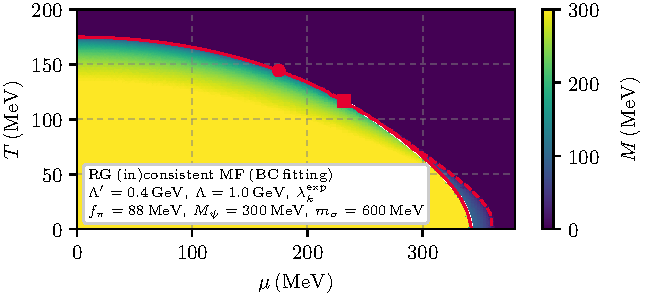
\includegraphics[width=11cm]{qmm/figures/eMFA_QMMCDW_PD_BC_04_10_88_300_600.pdf}
	}% Graphics
	[]
	{%
	\qmm{} phase diagram at $\Lambda=1\, \GeV$ with inhomogeneous window marked in red and homogeneous phase boundary (in white), which would occur if one were to disregard inhomogeneous condensation.
	Solid (dashed/dash-dotted) lines mark first-order (second-order) phase transitions.
	The dot marks the inhomogeneous \lp{} while the square marks the homogeneous \cp{}.
	All model parameters are included in the figure and the color map shows the magnitude of the quark mass parameter $M$.
	}%
	{fig:eMFA1}
\section{RG-consistent mean-field results}\label{sec:cdwmf}
As discussed in \cref{paragraph:introInhomoQMM} at the time we derived \cref{eq:cdwFlow}, we did not have the appropriate tools to numerically solve it. So in a first step we focused, before we got ``distracted'' by our studies in \dzero{} and \dtwo{}, on mean-field studies with this flow equation. Disregarding the novel contributions of the bosons the equation becomes an integral equation, \cf{} our discussion in \cref{chap:GN}, which can be integrated in \rgscale{} at wish symbolically. This allows for a direct application of the construction principles outlined in \cref{subsubsec:rgcICS}.

We chose the exponential regulator~\eqref{eq:rexp} for explicit numerical integration~\cite{cubature:2020} and subsequent repeated, local, numerical minimization~\cite{Nelder:1965} of the integrated flow equation \cref{eq:cdwFlow} using my \Cpp{} code~\cite{Steil:2023QMcpp}.
The phase boundaries have been obtained with the help of a block-structured adaptive mesh refinement algorithm, which I implemented for the efficient computation of these phase diagrams and the precise detection of lines of interest, without the need of explicit bisection. Details can be found in the \Cpp{} code~\cite{Steil:2023QMcpp} and its documentation.

While we are ultimately interested in an application of the \qmm{} as a \loeft{} theory in the context of \cref{subsec:chiralLEFT}, for this work we did not consider such a setup. We choose the standard bottom-up approach of many mean-field and \frg{} studies a like and fitted \ir{} observables to fix our model parameters. We choose a \textit{``sombrero''}-type (symmetric double-well) potential, \cf{} \cref{subsubsec:sc2}, as initial condition. Tuning its two parameters and the Yukawa coupling $h$ in vacuum to fix the bare pion decay constant $f_\pi$ to its common reference value in the chiral limit, \viz{} $f_\pi=88\,\MeV$, the curvature mass of the $\sigma$-meson to $m_\sigma=600\, \MeV$ and the quark mass parameter $M_\psi=300\,\MeV$.
We did so in an \rgct{} setting fixing those parameters at a relatively low model reference scale $\Lambda'=0.4\,\GeV$ and used the \frg{} flow as described in \cref{subsubsec:rgcICS} to construct a \uv{} completion \dash{} hence allow for a study not plagued by regularization artifacts. The resulting phase diagram constructing the completion up to $\Lambda=1\, \GeV$ is shown in \cref	{fig:eMFA1}

With \cref{fig:eMFA2} we show the corresponding situation using $\Lambda'=\Lambda=0.4\,\GeV$ and thus a situation without a proper \uv{} completion.
As one would expect we find an extreme violation of \rgcy{} at $T>0$ and the results basically loose complete predictive power for $\mu^2+\piu^2 T^2>\Lambda^2$ which we made out as a rough estimate. At these large external scales the initial scale $\Lambda=0.4\,\GeV$ is just too low in this case. This highlights the need for a proper \rgct{} \uv{} completion when using small $\Lambda'$.
\customWidthFigure%
	{%
	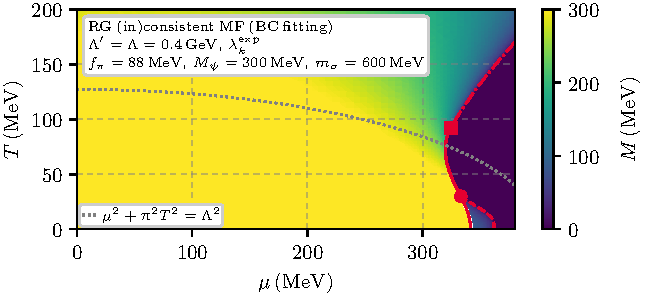
\includegraphics[width=11cm]{qmm/figures/eMFA_QMMCDW_PD_BC_04_04_88_300_600.pdf}
	}% Graphics
	[]
	{%
	Same as \cref{fig:eMFA1} but for lower $\Lambda'=\Lambda=0.4\, \GeV$. With the gray-dotted line ${\mu^2+\piu^2T^2=\Lambda^2}$ we mark an \aposteriori{} estimate for the range of validity of this computation.
	}%
	{fig:eMFA2}

We summarize the situation with \cref{fig:eMFA3} overlaying four results ranging  from $\Lambda=0.4\,\GeV$ up to $\Lambda=5\,\GeV$ all the while keeping $\Lambda'=0.4\,\GeV$. The difference between the results at $1\,\GeV$ and $5\,\GeV$ is rather small signaling that we are approaching \rgcy{} in the entire thermodynamic range considered.
We find a stable, persistent but rather small inhomogeneous phase ending in a \lp{} where \hbp{}, \ip{}, and \symp{} meet and beyond which we observe a second-order phase transition between \hbp{} and \symp{} as usual in the chiral limit in such models.

Using \rgcy{} as a guiding principle to construct proper \uv{} completions in \mf{} computations is a very elegant way to remove cutoff artifacts and focus on other issues, like, \eg{}, renormalization and/or parameter fitting.

Before discussing issues related to renormalization in the present approach, we want to comment on one particular limit. In a \rgct{} \mf{} computation it is technically possible to set $\Lambda'=0$ and thus \dash{} from an \frg{} perspective \dash{} fixing the \ea{} in the \ir{} without considering any vacuum fluctuations from the flow whatsoever. When doing this with the classical initial condition this effectively entails disregarding all fermionic quantum fluctuations, only allowing for thermodynamic ones. With a sufficiently large $\Lambda$ or even $\Lambda\rightarrow\infty$ we are thus able to recover the \textit{standard mean-field} result of \cref{fig:QMMsMFAref} in \cref{fig:sMFArg}\footnote{The only small quantitative difference stemming from the fact that in \ccite{Adhikari:2017ydi} $f_\pi=93\,\MeV$ is used while we fix $f_\pi=88\,\MeV$.}.\clearpage

\customWidthFigure%
	{%
	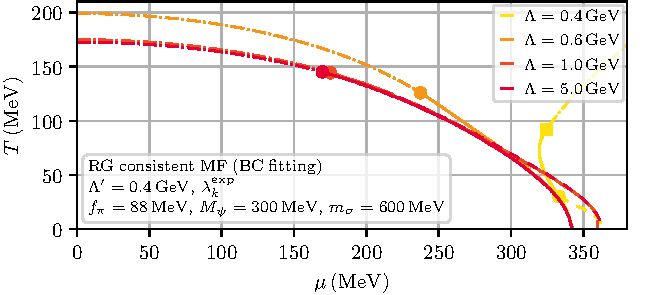
\includegraphics[width=11cm]{qmm/figures/eMFA_QMMCDW_PD_BC_04_all_88_300_600.pdf}
	}% Graphics
	[]
	{%
		Same as \cref{fig:eMFA1} but for increasing $\Lambda$: moving towards \rgcy{} from $\Lambda=0.4\,\GeV$ up to $\Lambda=5\,\GeV$ all the while keeping $\Lambda'=0.4\,\GeV$.
	}%
	{fig:eMFA3}
\customWidthFigure%
	{%
	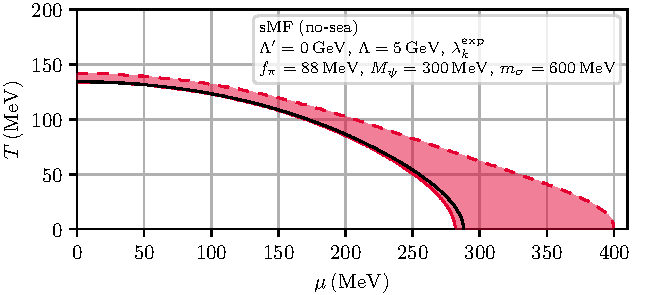
\includegraphics[width=11cm]{qmm/figures/sMFA_QMMCDW_PD_BC_0_5_88_300_600.pdf}
	}% Graphics
	[]
	{%
		Recovering the \textit{standard mean-field/no-sea} (sMF) result of \cref{fig:QMMsMFAref} with a \rgct{} reconstruction with $\Lambda'=0$ and $\Lambda=5\,\GeV$.
		The black line is the homogeneous phase boundary, the red lines and shaded area mark the inhomogeneous phase, and the solid (dashed) lines are first-(second-)order phase transitions.
	}%
	{fig:sMFArg}
\FloatBarrier
\subsection{Renormalized mean-field, parameter fitting, and \Poincare{} invariance}\label{subsec:renomMF}
Within this subsection we want to comment on important observations when it comes to renormalization in the present \mf{} context. One can consider the \qmm{} as a renormalizable \qft{} on its own and it is possible to renormalize it, \ie{}, remove all cutoffs and for these simple fermionic one-loop computations even all scheme-dependencies. The result for the inhomogeneous phase diagram in such a scenario is presented in \cref{fig:QMMrMFAref}, which was computed using dimensional regularization in the original \ccite{Adhikari:2017ydi}, but can be exactly reproduced by other regularization schemes like Pauli-Villars, see, \eg{}, \ccite{Carignano:2014jla}.

From the present perspective of the \qmm{} as a \loeft{} such a renormalization with a quartic potential in the limit $\Lambda\rightarrow\infty$ makes little sense.
It would however seem dishonest not to comment on the renormalization of the \qmm{} in the present setup as a consistency check in the spirit of all the other consistency checks discussed in this thesis.

\customWidthFigure%
	[!t]%
	{%
	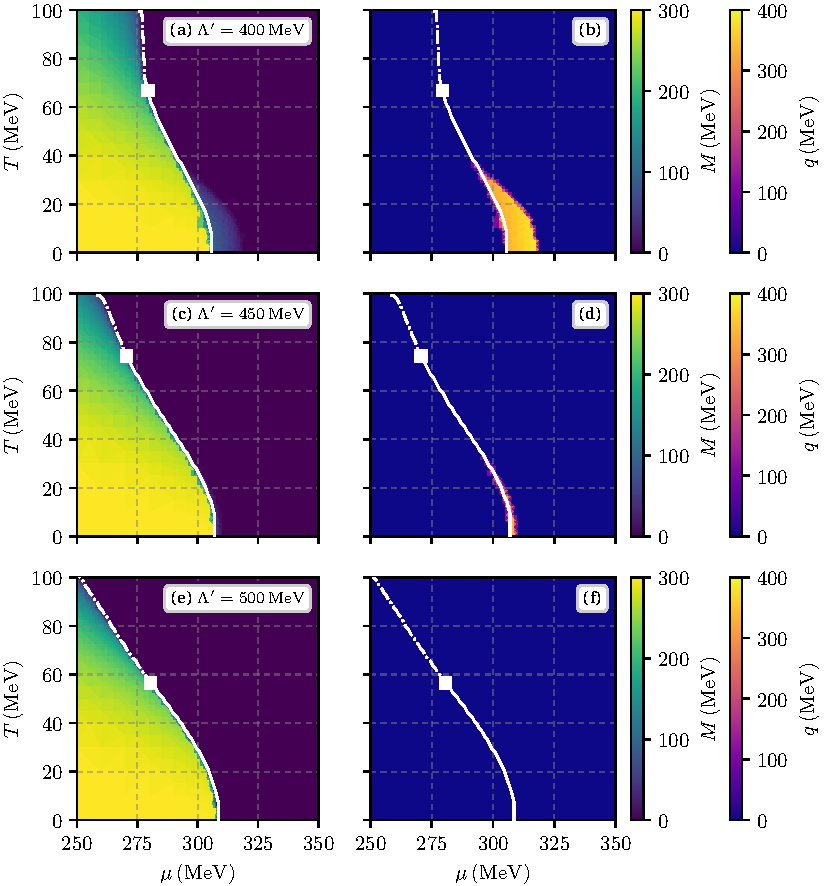
\includegraphics[width=\fullWidthFigureWidth]{qmm/figures/eMFAinhomo.pdf}
	}% Graphics
	[fig:eMFAinhomo_consistency_check400M,fig:eMFAinhomo_consistency_check400q,fig:eMFAinhomo_consistency_check450M,fig:eMFAinhomo_consistency_check450q,fig:eMFAinhomo_consistency_check500M,fig:eMFAinhomo_consistency_check500q]% Sublabels
	{%
		Starting at $\Lambda'=0.4\,\GeV$, \cf{} \cref{fig:eMFA2}, we increase $\Lambda'$ in increments of $0.05\,\GeV$ from top to bottom and observe the disappearance of the inhomogeneous window while fixing $\Lambda'=\Lambda$. The color map on the right (left) shows the magnitude of the quark mass parameter $M$ (\cdw{} wave vector $q$).
	}%Caption
	{fig:eMFAinhomo_consistency_check}%Label
\Cref{fig:eMFAinhomo_consistency_check} shows the immediate failure of this consistency check as we do not find any inhomogeneous phases for $\Lambda'\smallergtrsim 500\,\MeV$. The reason for this is however understood, see, \eg{}, \ccite{PhysRevD.94.034023} for the specific context here, and is quite general. When we fit our parameters to bare quantities, while considering fluctuations in the effective potential we incorporate fluctuations in an inconsistent way. For some observables and applications this might not be an issue, for the renormalized inhomogeneous phase diagram it is however a massive one~\cite{PhysRevD.94.034023,Carignano:2014jla}. One has to fit renormalized quantities: for the \qmm{} the renormalized pion decay constant and the pole mass of the sigma meson not its curvature mass. These can be computed on \lpa{}-level (mean-field being one further simplification) by evaluating the flow of the corresponding two-point functions, \cf{} our related discussion in \cref{sec:gnInfInhomo} and \cref{app:GNtwopt}. While the flow of the two-point function has no direct feedback into the \lpa{} flow it generates non-trivial contributions to the two-point functions.

In an attempt to sufficiently improve our parameter fitting a new issue arose, which we also wondered about in \cref{paragraph:comment_on_the_regulators} for the \gnym{}.
Our choice of regulator breaks (Euclidean) \Poincare{} invariance explicitly for all finite $\Lambda$, which is especially apparent in vacuum, where we are now trying to fit observables by computing wave-function renormalization factors and pole masses. We observe a splitting in the wave-function renormalization due to our regulator choice which spoils our results. We however found a solution for this problem by introducing appropriate counter terms in the \uv{} to account and correct for this splitting in the \ir{}, see, \eg{}, \ccite{Braun:2017srn,Pawlowski:2017gxj} for comments on such Ward identities.
Using two counter terms and fixing $1=Z_\pi^{||}=Z_\pi^\perp$ in the \ir{} seems to yield the best results at finite $\Lambda$. Preliminary tests show that one approaches the reference values of the renormalized limit as $\Lambda$ is increased. It seems however that with our exponential regulator this approach is rather slow. We have chosen this regulator to increase the performance of our numerical integration of the \cdw{} eigenvalues, which worked out well but especially for considerations of renormalization one should probably explore other options, \cf{} \ccite{Zorbach:2024zjx}.

With a remark in this direction we will finish this chapter: the flow \cref{eq:cdwFlow} for the \cdw{} for arbitrary regulator shape functions involves genuine two-dimensional integrals which is the main contributor to the numerical cost of these \mf{} computations. Numerical evaluating these integrals when studying the \frg{} flow with bosonic fluctuations in our developed \cfd{} context, seems like a daunting task: we have our volume cells in field direction, our flow in \rgtime{}, the wave vector of the \cdw{} as an additional minimization parameter and the $\mu$-$T$-plane to raster. A careful consideration of the angle-dependence in the eigenvalues \eqref{eq:cdwEfq} and \eqref{eq:cdwEb03q} of the \cdw{} might allow for an analytic evaluation for Litim-type regulators, which should definitely be considered when implementing the \lpa{} flow \cref{eq:cdwFlow}.
